\documentclass{ximera}

\title{Practice for Linearization and Stability}

%\auor{Matthew Charnley and Jason Nowell}
\usepackage[margin=1.5cm]{geometry}
\usepackage{indentfirst}
\usepackage{sagetex}
\usepackage{lipsum}
\usepackage{amsmath}
\usepackage{mathrsfs}


%%% Random packages added without verifying what they are really doing - just to get initial compile to work.
\usepackage{tcolorbox}
\usepackage{hypcap}
\usepackage{booktabs}%% To get \toprule,\midrule,\bottomrule etc.
\usepackage{nicefrac}
\usepackage{caption}
\usepackage{units}

% This is my modified wrapfig that doesn't use intextsep
\usepackage{mywrapfig}
\usepackage{import}



%%% End to random added packages.


\graphicspath{
    {./figures/}
    {./../figures/}
    {./../../figures/}
}
\renewcommand{\log}{\ln}%%%%
\DeclareMathOperator{\arcsec}{arcsec}
%% New commands


%%%%%%%%%%%%%%%%%%%%
% New Conditionals %
%%%%%%%%%%%%%%%%%%%%


% referencing
\makeatletter
    \DeclareRobustCommand{\myvref}[2]{%
      \leavevmode%
      \begingroup
        \let\T@pageref\@pagerefstar
        \hyperref[{#2}]{%
	  #1~\ref*{#2}%
        }%
        \vpageref[\unskip]{#2}%
      \endgroup
    }%

    \DeclareRobustCommand{\myref}[2]{%
      \leavevmode%
      \begingroup
        \let\T@pageref\@pagerefstar
        \hyperref[{#2}]{%
	  #1~\ref*{#2}%
        }%
      \endgroup
    }%
\makeatother

\newcommand{\figurevref}[1]{\myvref{Figure}{#1}}
\newcommand{\figureref}[1]{\myref{Figure}{#1}}
\newcommand{\tablevref}[1]{\myvref{Table}{#1}}
\newcommand{\tableref}[1]{\myref{Table}{#1}}
\newcommand{\chapterref}[1]{\myref{chapter}{#1}}
\newcommand{\Chapterref}[1]{\myref{Chapter}{#1}}
\newcommand{\appendixref}[1]{\myref{appendix}{#1}}
\newcommand{\Appendixref}[1]{\myref{Appendix}{#1}}
\newcommand{\sectionref}[1]{\myref{\S}{#1}}
\newcommand{\subsectionref}[1]{\myref{subsection}{#1}}
\newcommand{\subsectionvref}[1]{\myvref{subsection}{#1}}
\newcommand{\exercisevref}[1]{\myvref{Exercise}{#1}}
\newcommand{\exerciseref}[1]{\myref{Exercise}{#1}}
\newcommand{\examplevref}[1]{\myvref{Example}{#1}}
\newcommand{\exampleref}[1]{\myref{Example}{#1}}
\newcommand{\thmvref}[1]{\myvref{Theorem}{#1}}
\newcommand{\thmref}[1]{\myref{Theorem}{#1}}


\renewcommand{\exampleref}[1]{ {\color{red} \bfseries Normally a reference to a previous example goes here.}}
\renewcommand{\figurevref}[1]{ {\color{red} \bfseries Normally a reference to a previous figure goes here.}}
\renewcommand{\tablevref}[1]{ {\color{red} \bfseries Normally a reference to a previous table goes here.}}
\renewcommand{\Appendixref}[1]{ {\color{red} \bfseries Normally a reference to an Appendix goes here.}}
\renewcommand{\exercisevref}[1]{ {\color{red} \bfseries Normally a reference to a previous exercise goes here.}}



\newcommand{\R}{\mathbb{R}}

%% Example Solution Env.
\def\beginSolclaim{\par\addvspace{\medskipamount}\noindent\hbox{\bf Solution:}\hspace{0.5em}\ignorespaces}
\def\endSolclaim{\par\addvspace{-1em}\hfill\rule{1em}{0.4pt}\hspace{-0.4pt}\rule{0.4pt}{1em}\par\addvspace{\medskipamount}}
\newenvironment{exampleSol}[1][]{\beginSolclaim}{\endSolclaim}

%% General figure formating from original book.
\newcommand{\mybeginframe}{%
\begin{tcolorbox}[colback=white,colframe=lightgray,left=5pt,right=5pt]%
}
\newcommand{\myendframe}{%
\end{tcolorbox}%
}

%%% Eventually return and fix this to make matlab code work correctly.
%% Define the matlab environment as another code environment
%\newenvironment{matlab}
%{% Begin Environment Code
%{ \centering \bfseries Matlab Code }
%\begin{code}
%}% End of Begin Environment Code
%{% Start of End Environment Code
%\end{code}
%}% End of End Environment Code


% this one should have a caption, first argument is the size
\newenvironment{mywrapfig}[2][]{
 \wrapfigure[#1]{r}{#2}
 \mybeginframe
 \centering
}{%
 \myendframe
 \endwrapfigure
}

% this one has no caption, first argument is size,
% the second argument is a larger size used for HTML (ignored by latex)
\newenvironment{mywrapfigsimp}[3][]{%
 \wrapfigure[#1]{r}{#2}%
 \centering%
}{%
 \endwrapfigure%
}
\newenvironment{myfig}
    {%
    \begin{figure}[h!t]
        \mybeginframe%
        \centering%
    }
    {%
        \myendframe
    \end{figure}%
    }


% graphics include
\newcommand{\diffyincludegraphics}[3]{\includegraphics[#1]{#3}}
\newcommand{\myincludegraphics}[3]{\includegraphics[#1]{#3}}
\newcommand{\inputpdft}[1]{\subimport*{../figures/}{#1.pdf_t}}


%% Not sure what these even do? They don't seem to actually work... fun!
%\newcommand{\mybxbg}[1]{\tcboxmath[colback=white,colframe=black,boxrule=0.5pt,top=1.5pt,bottom=1.5pt]{#1}}
%\newcommand{\mybxsm}[1]{\tcboxmath[colback=white,colframe=black,boxrule=0.5pt,left=0pt,right=0pt,top=0pt,bottom=0pt]{#1}}
\newcommand{\mybxsm}[1]{#1}
\newcommand{\mybxbg}[1]{#1}

%%% Something about tasks for practice/hw?
\usepackage{tasks}
\usepackage{footnote}
\makesavenoteenv{tasks}


%% For pdf only?
\newcommand{\diffypdfversion}[1]{#1}


%% Kill ``cite'' and go back later to fix it.
\renewcommand{\cite}[1]{}


%% Currently we can't really use index or its derivatives. So we are gonna kill them off.
\renewcommand{\index}[1]{}
\newcommand{\myindex}[1]{#1}







\begin{document}
\begin{abstract}
Why?
\end{abstract}
\maketitle


\begin{exercise}
    Sketch the phase plane vector field for:
    \begin{itemize}
        \item $x'=x^2$, \enspace $y'=y^2$,
        \item $x'=(x-y)^2$, \enspace $y'=-x$,
        \item $x'=e^y$, \enspace $y'=e^x$.
    \end{itemize}
\end{exercise}
%\comboSol
%{%
%a)~\parbox[c]{1.4in}{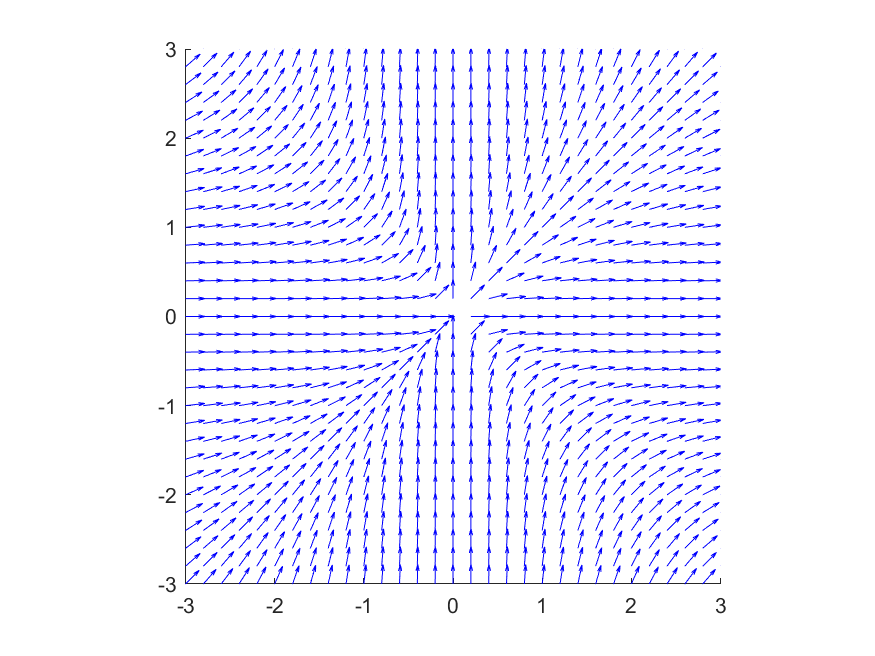
\includegraphics[width=1.4in]{Images/sysslopex2y2.png}} \quad b)~\parbox[c]{1.4in}{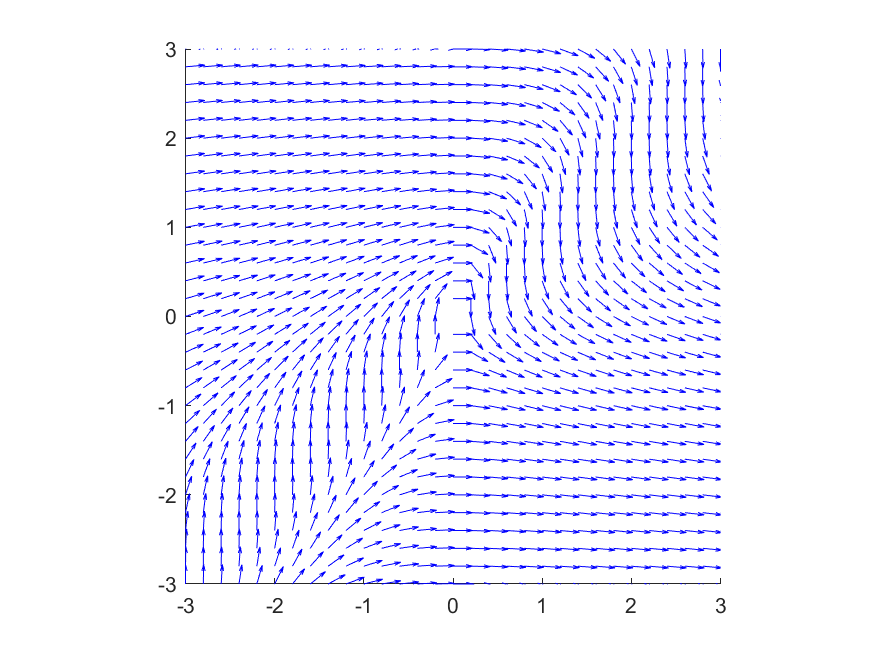
\includegraphics[width=1.4in]{Images/sysslopexmy2mx.png}} \quad c)~\parbox[c]{1.4in}{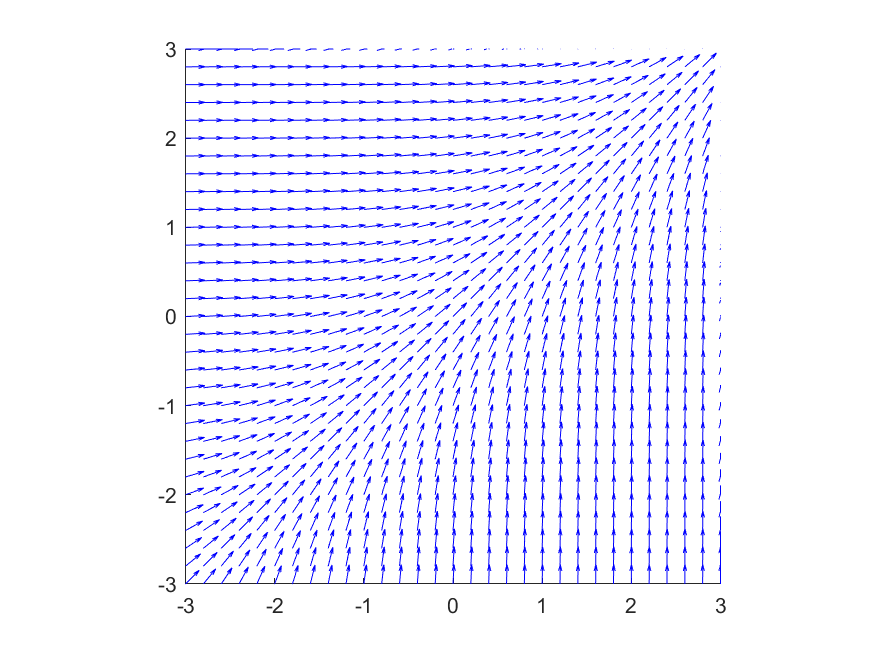
\includegraphics[width=1.4in]{Images/sysslopeeyex.png}}
%}

\begin{exercise}
    Match systems
    \begin{equation*}
        (i)\  x'=x^2, \enspace y'=y^2, \quad (ii)\  x'=xy, \enspace y'=1+y^2, \quad (iii)\  x'=\sin(\pi y), \enspace y'=x,
    \end{equation*}
    to the vector fields below.  Justify.
    \begin{itemize}
        \item \parbox[c]{1.75in}{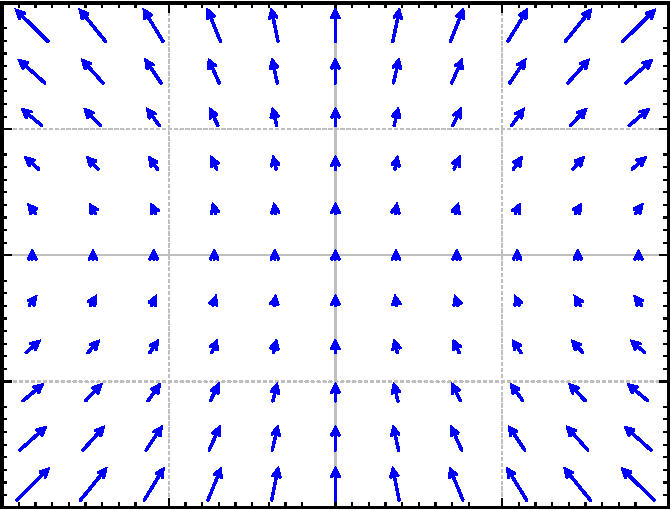
\includegraphics[width=1.75in]{../figures/nlin-exer-xy-1py2}}
            \begin{multipleChoice}
                \choice{i}
                \choice[correct]{ii}
                \choice{iii}
            \end{multipleChoice}
        \item \parbox[c]{1.75in}{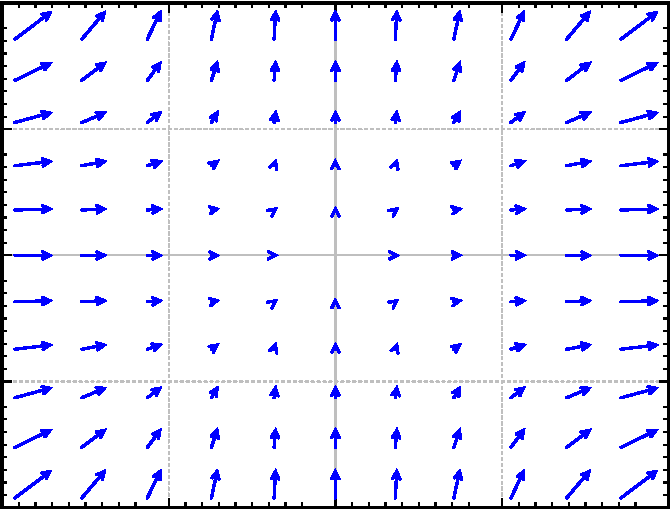
\includegraphics[width=1.75in]{../figures/nlin-exer-x2-y2}}
            \begin{multipleChoice}
                \choice[correct]{i}
                \choice{ii}
                \choice{iii}
            \end{multipleChoice}
        \item \parbox[c]{1.75in}{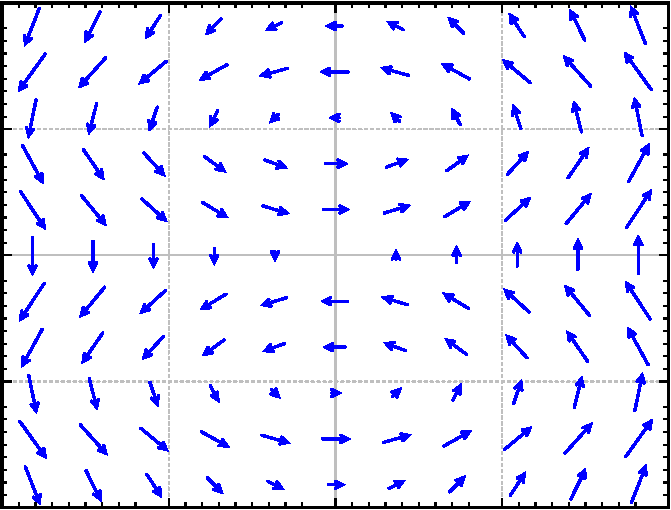
\includegraphics[width=1.75in]{../figures/nlin-exer-sinpiy-x}}
            \begin{multipleChoice}
                \choice{i}
                \choice{ii}
                \choice[correct]{iii}
            \end{multipleChoice}
    \end{itemize}
\end{exercise}
%\comboSol
%{%
%a)~ (ii) \quad b)~(i) \quad c)~(iii)
%}

\begin{exercise}%
    Match systems
    \begin{equation*}
        (i)\  x'=y^2, \enspace y'=-x^2, \quad (ii)\  x'=y, \enspace y'=(x-1)(x+1), \quad (iii)\  x'=y+x^2, \enspace y'=-x,
    \end{equation*}
    to the vector fields below.  Justify.
    \begin{itemize}
        \item \parbox[c]{1.75in}{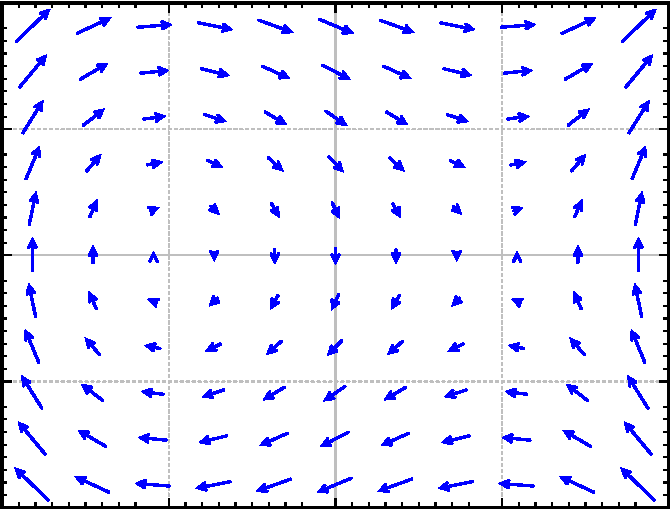
\includegraphics[width=1.75in]{../figures/nlin-exer-y-xm1xp1}}
            \begin{multipleChoice}
                \choice{i}
                \choice[correct]{ii}
                \choice{iii}
            \end{multipleChoice}
        \item \parbox[c]{1.75in}{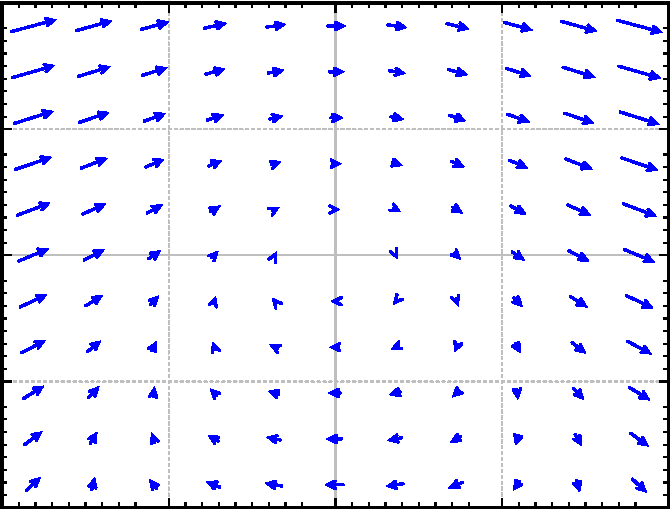
\includegraphics[width=1.75in]{../figures/nlin-exer-ypx2-mx}}
            \begin{multipleChoice}
                \choice{i}
                \choice{ii}
                \choice[correct]{iii}
            \end{multipleChoice}
        \item \parbox[c]{1.75in}{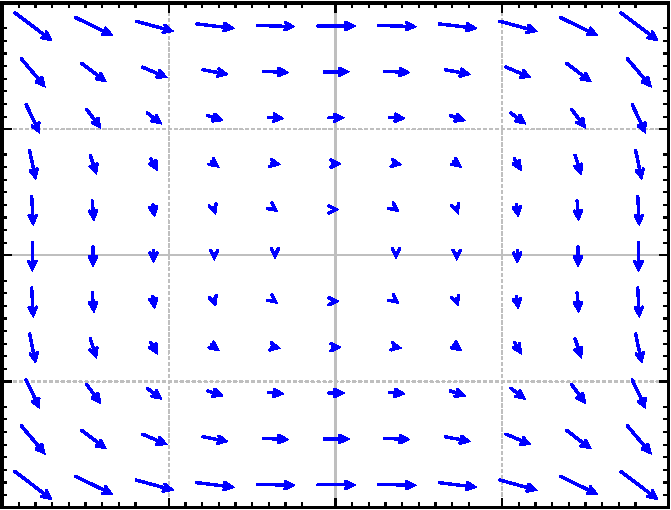
\includegraphics[width=1.75in]{../figures/nlin-exer-y2-mx2}}
            \begin{multipleChoice}
                \choice[correct]{i}
                \choice{ii}
                \choice{iii}
            \end{multipleChoice}
    \end{itemize}
\end{exercise}
%\exsol{%
%a)~(ii) \quad b)~(iii) \quad c)~(i)
%}


\begin{exercise}
    Find the critical points and linearizations of the following systems.
    \begin{itemize}
        \item $x'=x^2-y^2$, \enspace $y'=x^2+y^2-1$,\\
            Critical points: $\left(\pm \answer{\frac{\sqrt{2}}{2}}, \pm \answer{\frac{\sqrt{2}}{2}}\right)$. \\
            At $\left(+\answer{\frac{\sqrt{2}}{2}}, +\answer{\frac{\sqrt{2}}{2}}\right)$, linearization matrix is $\left[\begin{smallmatrix} \answer{\sqrt{2}} & -\sqrt{2} \\ \sqrt{2} & \answer{\sqrt{2}} \end{smallmatrix}\right]$. \\
            At $\left(+\answer{\frac{\sqrt{2}}{2}}, -\answer{\frac{\sqrt{2}}{2}}\right)$, linearization matrix is $\left[\begin{smallmatrix} \answer{\sqrt{2}} & \sqrt{2} \\ \answer{\sqrt{2}} & -\sqrt{2} \end{smallmatrix}\right]$.\\
            At $\left(-\answer{\frac{\sqrt{2}}{2}}, +\answer{\frac{\sqrt{2}}{2}}\right)$, linearization matrix is $\left[\begin{smallmatrix} -\answer{\sqrt{2}} & -\sqrt{2} \\ -\sqrt{2} & \answer{\sqrt{2}} \end{smallmatrix}\right]$. \\
            At $\left(-\answer{\frac{\sqrt{2}}{2}}, -\answer{\frac{\sqrt{2}}{2}}\right)$, linearization matrix is $\left[\begin{smallmatrix} -\sqrt{2} & \answer{\sqrt{2}} \\ -\answer{\sqrt{2}} & -\sqrt{2} \end{smallmatrix}\right]$. \\
        \item $x'=-y$, \enspace $y'=3x+yx^2$,\\
            Critical point: $\left(\answer{0},\answer{0}\right)$, linearization matrix $\left[\begin{smallmatrix} \answer{0} & \answer{-1} \\ \answer{3} & 0 \end{smallmatrix}\right]$\\
        \item $x'=x^2+y$, \enspace $y'=y^2+x$.\\
            Critical points: $\left(\answer{0},\answer{0}\right)$ and $\left(\answer{-1}, \answer{-1}\right)$. \\
            At $\left(\answer{0},\answer{0}\right)$, linearization matrix is $\left[\begin{smallmatrix} \answer{0} & 1 \\ \answer{1} & 0 \end{smallmatrix}\right]$. \\
            At $\left(\answer{-1}, \answer{-1}\right)$, linearization matrix is $\left[\begin{smallmatrix} \answer{-2} & \answer{1} \\ 1 & \answer{-2} \end{smallmatrix}\right]$\\
    \end{itemize}
\end{exercise}
%\comboSol
%{%
%a)~ Critical points: $\left(\pm \frac{\sqrt{2}}{2}, \pm \frac{\sqrt{2}}{2}\right)$. At $\left(\frac{\sqrt{2}}{2}, \frac{\sqrt{2}}{2}\right)$, linearization matrix is $\left[\begin{smallmatrix} \sqrt{2} & -\sqrt{2} \\ \sqrt{2} & \sqrt{2} \end{smallmatrix}\right]$. At $\left(\frac{\sqrt{2}}{2}, -\frac{\sqrt{2}}{2}\right)$, linearization matrix is $\left[\begin{smallmatrix} \sqrt{2} & \sqrt{2} \\ \sqrt{2} & -\sqrt{2} \end{smallmatrix}\right]$.
%At $\left(-\frac{\sqrt{2}}{2}, \frac{\sqrt{2}}{2}\right)$, linearization matrix is $\left[\begin{smallmatrix} -\sqrt{2} & -\sqrt{2} \\ -\sqrt{2} & \sqrt{2} \end{smallmatrix}\right]$. At $\left(-\frac{\sqrt{2}}{2}, -\frac{\sqrt{2}}{2}\right)$, linearization matrix is $\left[\begin{smallmatrix} -\sqrt{2} & \sqrt{2} \\ -\sqrt{2} & -\sqrt{2} \end{smallmatrix}\right]$. \\
%b)~Critical point: $(0,0)$, linearization matrix $\left[\begin{smallmatrix} 0 & -1 \\ 3 & 0 \end{smallmatrix}\right]$\\
%c)~Critical points: $(0,0)$ and $(-1, -1)$. At $(0,0)$, linearization matrix is $\left[\begin{smallmatrix} 0 & 1 \\ 1 & 0 \end{smallmatrix}\right]$. At $(-1, -1)$, linearization matrix is $\left[\begin{smallmatrix} -2 & 1 \\ 1 & -2 \end{smallmatrix}\right]$.
%}


\begin{exercise}%
    Find the critical points and linearizations of the following systems.
    \begin{itemize}
        \item $x'=\sin(\pi y)+(x-1)^2$, \enspace $y'=y^2-y$,\\
            Critical points $\left( \answer{1}, \answer{1} \right)$ and $\left( \answer{1}, \answer{0} \right)$.  \\
            At $\left( \answer{1}, \answer{1} \right)$ using $u = x - 1$, $v = y - 1$ the linearization is $u'= \answer{-\pi v}$, $v' = \answer{v}$.\\
            At $\left( \answer{1}, \answer{0} \right)$ using $u = x - 1$, $v = y$ the linearization is $u' = \answer{\pi v}$, $v' = \answer{-v}$.\\
        \item $x'=x+y+y^2$, \enspace $y'=x$,\\
            Critical points $\left( \answer{0},\answer{0} \right)$ and $\left(\answer{0}, \answer{-1} \right)$. \\
            For $\left( \answer{0}, \answer{0} \right)$, using $u=x$, $v=y$ the linearization is $u' = \answer{u + v}$, $v' = \answer{u}$. \\
            For $\left( \answer{0}, \answer{-1} \right)$, using $u = x$ and $v = y + 1$, the linearization is $u' = \answer{u - v}$, $v' = \answer{u}$\\
        \item $x'=(x-1)^2+y$, \enspace $y'=x^2+y$.\\
            Critical point $\left( \answer{\frac{1}{2}}, \answer{\frac{-1}{4}} \right)$. \\
            Using $u = x - \frac{1}{2}$, $v = y + \frac{1}{4}$ the linearization is $u' = \answer{-u + v}$, $v' = \answer{u + v}$.
    \end{itemize}
\end{exercise}
%\exsol{%
%a) Critical points $(1,1)$ and $(1,0)$.  At $(1,1)$ using $u=x-1$, $v=y-1$ the linearization is $u'=-\pi v$, $v'=v$.
%At $(1,0)$ using $u=x-1$, $v=y$ the linearization is
%$u'=\pi v$, $v'=-v$.\\
%b) Critical points $(0,0)$ and $(0, -1)$. For $(0,0)$, using $u=x$, $v=y$ the linearization is
%$u'=u+v$, $v'=u$. For $(0,-1)$, using $u = x$ and $v = y+1$, the linearization is $u' = u-v$, $v' = u$\\
%c) Critical point $(\frac{1}{2},\frac{-1}{4})$.  Using
%$u=x-\frac{1}{2}$, $v=y+\frac{1}{4}$ the linearization is
%$u'=-u+v$, $v'=u+v$.
%}

\begin{exercise}
    For the following systems, verify they have critical point at $(0,0)$, and find the linearization at $(0,0)$.
    \begin{itemize}
        \item $x'=x+2y+x^2-y^2$, \enspace $y'=2y-x^2$\\
            $\left[\begin{smallmatrix} \answer{1} & 2 \\ 0 & \answer{2} \end{smallmatrix}\right]$
        \item $x'=-y$, \enspace $y'=x-y^3$\\
            $\left[\begin{smallmatrix} \answer{1} & \answer{1} \\ 1 & \answer{0} \end{smallmatrix}\right]$
        \item* $x'=ax+by+f(x,y)$, $y'=cx+dy+g(x,y)$, 
            where $f(0,0) = 0$, $g(0,0) = 0$, and all first partial derivatives of $f$ and $g$ are also zero at $(0,0)$, that is, $\frac{\partial f}{\partial x}(0,0) = \frac{\partial f}{\partial y}(0,0) = \frac{\partial g}{\partial x}(0,0) = \frac{\partial g}{\partial y}(0,0) = 0$.\\
            $\left[\begin{smallmatrix} \answer{a} & \answer{b} \\ \answer{c} & \answer{d} \end{smallmatrix}\right]$.
    \end{itemize}
\end{exercise}
%\comboSol
%{%
%a)~ $\left[\begin{smallmatrix} 1 & 2 \\ 0 & 2 \end{smallmatrix}\right]$ \quad b)~ $\left[\begin{smallmatrix} 1 & 1 \\ 1 & 0 \end{smallmatrix}\right]$ \qquad c)~ $\left[\begin{smallmatrix} a & b \\ c & d \end{smallmatrix}\right]$.
%}

\begin{exercise}
    Take the system $x' = (x-2)(x+y)$, \ $y' = (y+3)(x-y)$.
    
    Find all critical points.\\
    $\left(\answer{0}, \answer{0}\right)$, $\left(\answer{2}, \answer{-3}\right)$, $\left(\answer{2}, \answer{2}\right)$, $\left(\answer{3}, \answer{-3}\right)$
    \begin{problem}
        Determine the linearization of this system around each of the critical points.\\
            $(0,0)$, $\left[\begin{smallmatrix} \answer{-2} & \answer{-2} \\ \answer{3} & -3 \end{smallmatrix}\right]$, \\ 
            $(2, -3)$, $\left[\begin{smallmatrix} -1 & \answer{0} \\ \answer{0} & \answer{1} \end{smallmatrix}\right]$, \\ 
            $(2, 2)$, $\left[\begin{smallmatrix} \answer{2} & \answer{0} \\ 5 & \answer{-5} \end{smallmatrix}\right]$, \\ 
            $(3, -3)$, $\left[\begin{smallmatrix} 1 & \answer{1} \\ \answer{0} & \answer{6} \end{smallmatrix}\right]$, \\
        \begin{problem}
            For each of the critical points, determine the behavior and classify the type of solution that the  \emph{linearized} system will have around that critical point. \\
            $(0,0)$,  \\
            \begin{multipleChoice}
                \choice{sink}
                \choice[correct]{Nodal sink}
                \choice{Saddle}
                \choice{Nodal Saddle}
                \choice{Source}
                \choice{Nodal Source}
            \end{multipleChoice}
            $(2, -3)$
            \begin{multipleChoice}
                \choice{sink}
                \choice{Nodal sink}
                \choice[correct]{Saddle}
                \choice{Nodal Saddle}
                \choice{Source}
                \choice{Nodal Source}
            \end{multipleChoice}
            $(2, 2)$
            \begin{multipleChoice}
                \choice{sink}
                \choice{Nodal sink}
                \choice[correct]{Saddle}
                \choice{Nodal Saddle}
                \choice{Source}
                \choice{Nodal Source}
            \end{multipleChoice}
            $(3, -3)$
            \begin{multipleChoice}
                \choice{sink}
                \choice{Nodal sink}
                \choice{Saddle}
                \choice{Nodal Saddle}
                \choice{Source}
                \choice[correct]{Nodal Source}
            \end{multipleChoice}
        \end{problem}
    \end{problem}
\end{exercise}
%\comboSol
%{%
%$(0,0)$, $\left[\begin{smallmatrix} -2 & -2 \\ 3 & -3 \end{smallmatrix}\right]$, Nodal sink.\ $(2, -3)$, $\left[\begin{smallmatrix} -1 & 0 \\ 0 & 1 \end{smallmatrix}\right]$, Saddle. \ 
%$(2, 2)$, $\left[\begin{smallmatrix} 2 & 0 \\ 5 & -5 \end{smallmatrix}\right]$, Saddle.\ 
%$(3, -3)$, $\left[\begin{smallmatrix} 1 & 1 \\ 0 & 6 \end{smallmatrix}\right]$, Nodal source. 
%}

\begin{exercise}
    Take the system $x' = (x^2 - y)(x+3)$, \ $y' = (y-1)(x+y+1)$.
    Find all critical points.\\
    $\left(\answer{-1}, \answer{1}\right)$, $\left(\answer{1}, \answer{1}\right)$, $\left(\answer{-3}, \answer{1}\right)$, $\left(\answer{-3}, \answer{4}\right)$, $\left( \answer{-\frac{1}{2} + \frac{\sqrt{5}}{2}}, \answer{\frac{3}{2} - \frac{\sqrt{5}}{2}}\right)$, $\left( \answer{-\frac{1}{2} - \frac{\sqrt{5}}{2}}, \answer{\frac{3}{2} + \frac{\sqrt{5}}{2}}\right)$
    \begin{problem}
        Determine the linearization of this system around each of the critical points.\\
            $(-1,1)$, $\left[\begin{smallmatrix} \answer{-4} & \answer{-2} \\ 0 & \answer{-1} \end{smallmatrix}\right]$, \\
            $(1,1)$, $\left[\begin{smallmatrix} \answer{8} & \answer{-4} \\ \answer{0} & 1 \end{smallmatrix}\right]$, \\
            $(-3, 1)$, $\left[\begin{smallmatrix} \answer{8} & \answer{0} \\ 0 & \answer{-3} \end{smallmatrix}\right]$,  \\
            $(-3, 4)$, $\left[\begin{smallmatrix} 5 & \answer{0} \\ \answer{3} & \answer{3} \end{smallmatrix}\right]$, \\ 
            $\left( -\frac{1}{2} + \frac{\sqrt{5}}{2}, \frac{3}{2} - \frac{\sqrt{5}}{2}\right)$, $\left[\begin{smallmatrix} \answer{2\sqrt{5}} & \answer{-\frac{5}{2} - \frac{\sqrt{5}}{2}} \\ \answer{\frac{1}{2} - \frac{\sqrt{5}}{2}} & \frac{1}{2} - \frac{\sqrt{5}}{2} \end{smallmatrix}\right]$, \\
            $\left( -\frac{1}{2} - \frac{\sqrt{5}}{2}, \frac{3}{2} + \frac{\sqrt{5}}{2}\right)$, $\left[\begin{smallmatrix} -2\sqrt{5} & \answer{-\frac{5}{2} + \frac{\sqrt{5}}{2}} \\ \answer{\frac{1}{2} + \frac{\sqrt{5}}{2}} & \answer{\frac{1}{2} + \frac{\sqrt{5}}{2}} \end{smallmatrix}\right]$\\
        \begin{problem}
            For each of the critical points, determine the behavior and classify the type of solution that the  \emph{linearized} system will have around that critical point. \\
            $\left(\answer{-1}, \answer{1}\right)$,   \\
            \begin{multipleChoice}
                \choice{sink}
                \choice[correct]{Nodal sink}
                \choice{Saddle}
                \choice{Nodal Saddle}
                \choice{Source}
                \choice{Nodal Source}
            \end{multipleChoice}
            $\left(\answer{1}, \answer{1}\right)$, 
            \begin{multipleChoice}
                \choice{sink}
                \choice{Nodal sink}
                \choice{Saddle}
                \choice{Nodal Saddle}
                \choice{Source}
                \choice[correct]{Nodal Source}
            \end{multipleChoice}
            $\left(\answer{-3}, \answer{1}\right)$, 
            \begin{multipleChoice}
                \choice{sink}
                \choice{Nodal sink}
                \choice[correct]{Saddle}
                \choice{Nodal Saddle}
                \choice{Source}
                \choice{Nodal Source}
            \end{multipleChoice}
            $\left(\answer{-3}, \answer{4}\right)$, 
            \begin{multipleChoice}
                \choice{sink}
                \choice{Nodal sink}
                \choice{Saddle}
                \choice{Nodal Saddle}
                \choice{Source}
                \choice[correct]{Nodal Source}
            \end{multipleChoice}
            $\left( \answer{-\frac{1}{2} + \frac{\sqrt{5}}{2}}, \answer{\frac{3}{2} - \frac{\sqrt{5}}{2}}\right)$, 
            \begin{multipleChoice}
                \choice{sink}
                \choice{Nodal sink}
                \choice[correct]{Saddle}
                \choice{Nodal Saddle}
                \choice{Source}
                \choice{Nodal Source}
            \end{multipleChoice}
            $\left( \answer{-\frac{1}{2} - \frac{\sqrt{5}}{2}}, \answer{\frac{3}{2} + \frac{\sqrt{5}}{2}}\right)$ 
            \begin{multipleChoice}
                \choice{sink}
                \choice{Nodal sink}
                \choice[correct]{Saddle}
                \choice{Nodal Saddle}
                \choice{Source}
                \choice{Nodal Source}
            \end{multipleChoice}
        \end{problem}
    \end{problem}
\end{exercise}
%\comboSol
%{% 
%$(-1,1)$, $\left[\begin{smallmatrix} -4 & -2 \\ 0 & -1 \end{smallmatrix}\right]$, Nodal sink.\ $(1,1)$, $\left[\begin{smallmatrix} 8 & -4 \\ 0 & 1 \end{smallmatrix}\right]$, Nodal source.\ 
%$(-3, 1)$, $\left[\begin{smallmatrix} 8 & 0 \\ 0 & -3 \end{smallmatrix}\right]$, Saddle.\ 
%$(-3, 4)$, $\left[\begin{smallmatrix} 5 & 0 \\ 3 & 3 \end{smallmatrix}\right]$, Nodal Source.\ 
%$\left( -\frac{1}{2} + \frac{\sqrt{5}}{2}, \frac{3}{2} - \frac{\sqrt{5}}{2}\right)$, $\left[\begin{smallmatrix} 2\sqrt{5} & -\frac{5}{2} - \frac{\sqrt{5}}{2} \\ \frac{1}{2} - \frac{\sqrt{5}}{2} & \frac{1}{2} - \frac{\sqrt{5}}{2} \end{smallmatrix}\right]$, Saddle.\ 
%$\left( -\frac{1}{2} - \frac{\sqrt{5}}{2}, \frac{3}{2} + \frac{\sqrt{5}}{2}\right)$, $\left[\begin{smallmatrix} -2\sqrt{5} & -\frac{5}{2} + \frac{\sqrt{5}}{2} \\ \frac{1}{2} + \frac{\sqrt{5}}{2} & \frac{1}{2} + \frac{\sqrt{5}}{2} \end{smallmatrix}\right]$, Saddle.
%}

\begin{exercise}
    Take $x'=(x-y)^2$, \enspace $y'=(x+y)^2$. \\
    Find the set of critical points. $\left(\answer{0}, \answer{0}\right)$
    \begin{problem}
        Sketch a phase diagram and describe the behavior near the critical point(s) and find the linearization.\\
        Solutions move away from $\answer{0}$, generally above the line $y=\answer{x}$
        \begin{feedback}[correct]
            Is it helpful in understanding the system?
        \end{feedback}
    \end{problem}
\end{exercise}
%\comboSol
%{%
%a)~(0,0) \quad b)~Solutions move away from 0, generally above the line $y=x$ \quad c)~No. Linearization is 0.
%}

\begin{exercise}
    Take $x'=x^2$, \enspace $y'=x^3$.
    Find the set of critical points. $\left(\answer{0}, \answer{y}\right)$
    \begin{problem}
        Sketch a phase diagram and describe the behavior near the critical point(s) \\
        Generally curving \wordChoice{\choice[correct]{upward}\choice{downward}\choice{toward the x-axis.}} as $x$ gets bigger
        
        \begin{problem}
            Find the linearization.\\
            The linearization is $\answer{0}$.
            \begin{feedback}[correct]
                Is it helpful in understanding the system?
            \end{feedback}
        \end{problem}
    \end{problem}
\end{exercise}
%\comboSol
%{%
%a)~$(0,y)$ for any $y$. \quad b)~Generally curving upward as $x$ gets bigger \quad c)~No. Linearization is zero at any critical point.
%}


\begin{exercise}%
    The idea of critical points and linearization works in higher dimensions as well.  You simply make the Jacobian matrix bigger by adding more functions and more variables.  For the following system of 3 equations find the critical points and their linearizations:
    \begin{equation*}
        x' = x + z^2, \qquad y' = z^2-y, \qquad z' = z+x^2.
    \end{equation*}
\end{exercise}

%\exsol{%
%Critical points are $(0,0,0)$, and
%$(-1, 1, -1)$.
%The linearization at the origin using variables $u=x$, $v=y$, $w=z$ is
%$u' = u$, $v'=-v$, $z' = w$.
%The linearization at the point $(-1,1,-1)$ using variables $u=x+1$,
%$v=y-1$, $w=z+1$ is
%%$x=u-1$
%%$y=v+1$
%%$z=w-1$
%%$u' = u-1 + (w-1)^2$, $v' = (w-1)^2-v+1$, $w' = (w-1)+(u-1)^2$.
%%$u' = u + w^2-2w$, $v' = w^2-2w-v$, $w' = w+u^2-2u$
%$u'=u-2w$, $v'=-v-2w$, $w'=w-2u$.
%}

\begin{exercise}%
    Any two-dimensional non-autonomous system $x'=f(x,y,t)$, $y'=g(x,y,t)$ can be written as a three-dimensional autonomous system (three equations).  Write down this autonomous system using the variables $u$, $v$, $w$.\\
    $u' = f(u,v,w)$, $v'=g(u,v,w)$, $w' = \answer{1}$.
\end{exercise}
%\exsol{%
%$u' = f(u,v,w)$, $v'=g(u,v,w)$, $w' = 1$.
%}

\begin{exercise}
    For the systems below, find and classify the critical points, also indicate if the equilibria are stable, asymptotically stable, or unstable.
    \begin{itemize}
        \item $x'=-x+3x^2, y'=-y$
        \item $x'=x^2+y^2-1$, $y'=x$
        \item $x'=ye^x$, $y'=y-x+y^2$
    \end{itemize}
\end{exercise}
%\comboSol
%{%
%a)~$(0,0)$ nodal sink, asymptotically stable. $(1/3, 0)$ saddle, unstable.\\
%b)~$(0,1)$ saddle, unstable. $(0, -1)$ center, unknown, maybe stable. \\
%c)~$(0,0)$ spiral source, unstable. 
%}

\begin{exercise}%
    For the systems below, find and classify the critical points.
    \begin{itemize}
        \item $x'=-x+x^2$, $y'=y$
        \item $x'=y-y^2-x$, $y'=-x$
        \item $x'=xy$, $y'=x+y-1$
    \end{itemize}
\end{exercise}
%\exsol{%
%a) $(0,0)$: saddle (unstable), $(1,0)$: source (unstable), \qquad
%b) $(0,0)$: spiral sink (asymptotically stable), $(0,1)$: saddle (unstable), \qquad
%c) $(1,0)$: saddle (unstable), $(0,1)$: improper nodal source (unstable)
%}

\begin{exercise}
    Find and classify all critical points of the system
    \[ 
        \frac{dx}{dt} = (x+1)(x-y+3) \qquad \frac{dy}{dt} = (x-2)(x-y) .
    \]
    $\left(\answer{-1}, \answer{-1}\right)$ Which is a:
    \begin{multipleChoice}
        \choice{saddle}
        \choice{source}
        \choice{sink}
        \choice{spiral saddle}
        \choice{spiral source}
        \choice{spiral sink}
        \choice{nodal saddle}
        \choice{nodal source}
        \choice{nodal sink}
        \choice{improper nodal saddle}
        \choice[correct]{improper nodal source}
        \choice{improper nodal sink}
    \end{multipleChoice}
    And it is \wordChoice{\choice{stable}\choice{Asymptotically stable}\choice[correct]{unstable}}.\\
    $\left(\answer{2}, \answer{5}\right)$ Which is a:
    \begin{multipleChoice}
        \choice[correct]{saddle}
        \choice{source}
        \choice{sink}
        \choice{spiral saddle}
        \choice{spiral source}
        \choice{spiral sink}
        \choice{nodal saddle}
        \choice{nodal source}
        \choice{nodal sink}
        \choice{improper nodal saddle}
        \choice{improper nodal source}
        \choice{improper nodal sink}
    \end{multipleChoice}
    And it is \wordChoice{\choice{stable}\choice{Asymptotically stable}\choice[correct]{unstable}}.
\end{exercise}
%\comboSol
%{%
%$(-1, -1)$, improper nodal source, unstable. $(2,5)$, saddle, unstable.
%}

\begin{exercise}
    Find and classify all critical points of the system
    \[ 
        \frac{dx}{dt} = x^2 - y^2 \qquad \frac{dy}{dt} = (x+4)(y-2) .
    \]
    $\left(\answer{-4}, \answer{4}\right)$ Which is a:
    \begin{multipleChoice}
        \choice{saddle}
        \choice{source}
        \choice{sink}
        \choice{spiral saddle}
        \choice{spiral source}
        \choice{spiral sink}
        \choice{nodal saddle}
        \choice{nodal source}
        \choice{nodal sink}
        \choice{improper nodal saddle}
        \choice{improper nodal source}
        \choice[correct]{improper nodal sink}
    \end{multipleChoice}
    And it is \wordChoice{\choice{stable}\choice[correct]{Asymptotically stable}\choice{unstable}}.\\
    $\left(\answer{-4}, \answer{-4}\right)$ Which is a:
    \begin{multipleChoice}
        \choice{saddle}
        \choice{source}
        \choice{sink}
        \choice{spiral saddle}
        \choice{spiral source}
        \choice[correct]{spiral sink}
        \choice{nodal saddle}
        \choice{nodal source}
        \choice{nodal sink}
        \choice{improper nodal saddle}
        \choice{improper nodal source}
        \choice{improper nodal sink}
    \end{multipleChoice}
    And it is \wordChoice{\choice{stable}\choice[correct]{Asymptotically stable}\choice{unstable}}.\\
    $\left(\answer{-2}, \answer{2}\right)$ Which is a:
    \begin{multipleChoice}
        \choice[correct]{saddle}
        \choice{source}
        \choice{sink}
        \choice{spiral saddle}
        \choice{spiral source}
        \choice{spiral sink}
        \choice{nodal saddle}
        \choice{nodal source}
        \choice{nodal sink}
        \choice{improper nodal saddle}
        \choice{improper nodal source}
        \choice{improper nodal sink}
    \end{multipleChoice}
    And it is \wordChoice{\choice{stable}\choice{Asymptotically stable}\choice[correct]{unstable}}.\\
    $\left(\answer{-2}, \answer{2}\right)$ Which is a:
    \begin{multipleChoice}
        \choice{saddle}
        \choice{source}
        \choice{sink}
        \choice{spiral saddle}
        \choice{spiral source}
        \choice{spiral sink}
        \choice{nodal saddle}
        \choice[correct]{nodal source}
        \choice{nodal sink}
        \choice{improper nodal saddle}
        \choice{improper nodal source}
        \choice{improper nodal sink}
    \end{multipleChoice}
    And it is \wordChoice{\choice{stable}\choice{Asymptotically stable}\choice[correct]{unstable}}.
\end{exercise}
%\comboSol
%{%
%$(-4, 4)$, improper nodal sink, asymptotically stable. $(-4, -4)$, spiral sink, asymptotically stable. $(-2, 2)$, saddle, unstable. $(2,2)$, nodal source, unstable.
%}


\begin{exercise}
    Find and classify the critical point(s) of $x' = -x^2$, $y' = -y^2$.\\
    $\left(\answer{0}, \answer{0}\right)$ which is \wordChoice{\choice{stable}\choice{Asymptotically stable}\choice[correct]{unstable}}.
\end{exercise}
%\comboSol
%{%
%$(0,0)$ Unstable. Everything moves downward, so if either component is negative, the solution converges away from $(0,0)$.
%}


\begin{exercise}
    Suppose $x'=-xy$, $y'=x^2-1-y$.
    \begin{itemize}
        \item Show there are two spiral sinks at $(-1,0)$ and $(1,0)$.
        \item For any initial point of the form $(0,y_0)$, find the trajectory.
        \item Can a trajectory starting at $(x_0,y_0)$ where $x_0 > 0$ spiral into the critical point at $(-1,0)$?  Why or why not?
    \end{itemize}
\end{exercise}


%\comboSol
%{%
%b)~The solution will converge (exponentially) to $(0, -1)$. \quad c)~ No, it can not cross another solution curve.
%}

\begin{exercise} \label{exercise:increasing}
    In the example $x'=y$, $y'=y^3-x$ show that for any trajectory, the distance from the origin is an increasing function. Conclude that the origin behaves like is a spiral source. Hint: Consider 
    $f(t) = {\bigl(x(t)\bigr)}^2 + {\bigl(y(t)\bigr)}^2$ and show it has positive derivative.\\
    $\answer{2r}\frac{dr}{dt} = \answer{2y^4} > 0$
\end{exercise}
%\comboSol
%{%
%$2r\frac{dr}{dt} = 2y^4 > 0$
%}

\begin{exercise}
    Find and analyze all critical points of the system $x' = y$, $y' = -x - y^3$. Use the ideas from exercise \ref{exercise:increasing} to show that the solutions to this problem move towards the origin as $t$ grows.\\
    $\answer{2r}\frac{dr}{dt} = \answer{-2y^4} < 0$
\end{exercise}
%\comboSol
%{%
%$2r\frac{dr}{dt} = -2y^4 < 0$
%}

\begin{exercise}%
    Derive an analogous classification of critical points for equations in one dimension, such as $x'= f(x)$ based on the derivative.  A point $x_0$ is critical when $f(x_0) = 0$ and almost linear if in addition $f'(x_0) \not= 0$.  Figure out if the critical point is stable or unstable depending on the sign of $f'(x_0)$.  Explain.  Hint: see section \ref{auteq:section}.\\
    A critical point $x_0$ is stable if $f'(x_0) < \answer{0}$ and unstable when $f'(x_0) > \answer{0}$.
\end{exercise}
%\exsol{%
%A critical point $x_0$ is stable if $f'(x_0) < 0$ and unstable when $f'(x_0)
%> 0$.
%}

%
%\setcounter{exercise}{100}

\end{document}